\section{Annexes}


\subsection{Compléments sur l'analyse temps-fréquence} \label{ann:complement_t-f}

\thoughts{C'est un copier collé du premier jet du mémoire, c'est pas très cohérent avec le reste là tout de suite. Je la retoucherai plus tard.}
\\



\subsubsection{\wip Formalisme derrière la transformée en SA ou le problème de signaux réels et comment le résoudre} \label{sec:transfo_SA}

D'abord, du point de vue de l'analyse temps-fréquence, les signaux réels sont problématiques car leur spectre sont à symétrie hermitienne et leur  densité spectrale symétrique :
\begin{align*}
	\forall t\in\R,\ x(t)\in\R \quad &\Lr \quad \forall \nu\in\R,\ \fou{x}(-\nu) = \congu{\fou{x}(\nu)} \\
	&\Lr \quad \forall \nu\in\R,\ \densis(-\nu) = \densis(\nu)
\end{align*}
\skipl \\
Comme mentionné plus haut, cela implique que la fréquence moyenne de tout signal réel est nulle (intégrale d'une fonction impaire). Ce qui, en plus de ne pas être très instructif, n'est pas cohérent avec l'interprétation physique qu'on voudrait faire cette moyenne. Par exemple, si $\densis$ prend la forme ci-dessous (\cref{fig:densi_spec_sym}), alors il serait plus naturelle de demander à ce que la fréquence moyenne se trouve autour de \textbf{1,4}. De même, la largeur de bande spectrale ne correspond plus à l'étalement de chaque gaussienne, mais plutôt à leur espacement.
\\
\begin{figure}[h]\centering
	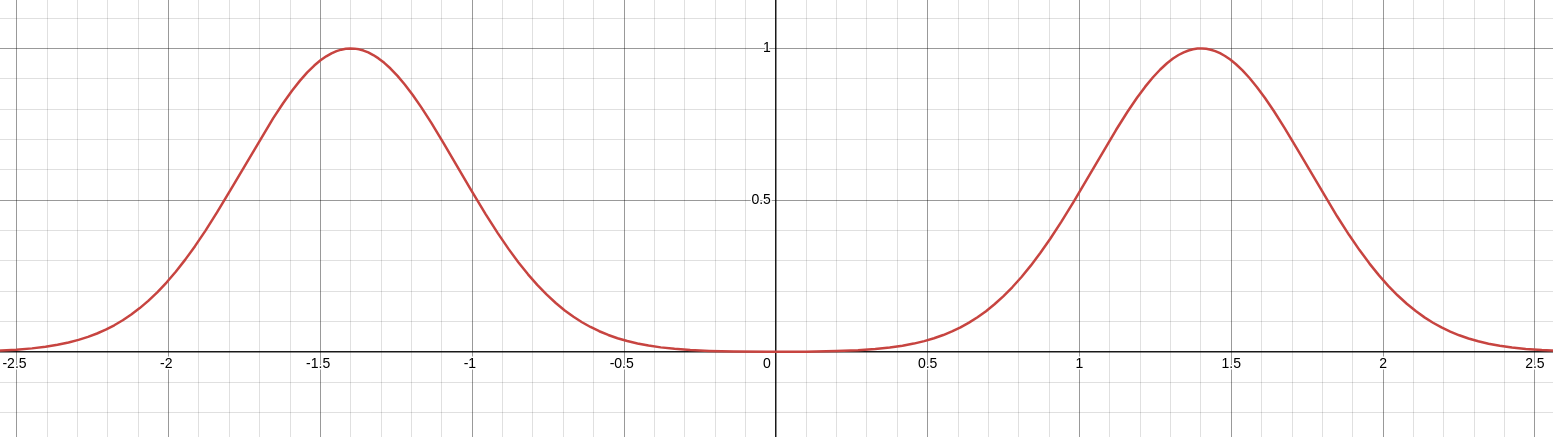
\includegraphics[width=0.9\textwidth]{fig/part-1/densi_spec_sym}
	\caption{Exemple de densité spectrale d'un signal réel \textbf{ESP A 1,4}}
	\label{fig:densi_spec_sym}
\end{figure}
\\
Même problème avec la covariance : sachant l'égalité des deux notions de fréquences moyenne (\cref{eq:esp_freq}, \cref{prop:mom_freq}), on peut définir la covariance temps-fréquence d'un signal $x$ par :
\begin{align*}
	\text{Cov}(x) \defeq \text{Cov}\big(t,\phi'(t) \big) 
	&= \esp[\densit]{t\phi'(t)} - \esp[\densit]{t} \esp[\densit]{\phi'(t)} \\
	&= \esp[\densit]{t\phi'(t)} - \esp[\densit]{t} \esp[\densis]{\nu}	
\end{align*}
\\
Ce coefficient est sensé mesurer une corrélation entre l'évolution d'un signal au cours du temps avec ses fréquences. S'il est réel, alors  $\text{Cov}(x)$ sera toujours nulle ; de là à en conclure que la fréquence instantanée de n'importe quel signal (réel) est toujours décorrélée du temps serait, pour le moins, insatisfaisant.
\\

Pour résoudre le problème, une méthode consiste à construire un nouveau signal $\SA{x}$ en supprimant les fréquences négatives de $x$ :
\[\mathcal{F}\big[\SA{x}\big] = 2\one_{\R^+}\fou{x}\]
où $\one_E$ est la fonction indicatrice sur l'ensemble $E$ et où le facteur 2 assure la conservation de l'énergie du signal. Cela mène à la définition :

\begin{definition}[Transformée de Hilbert et en SA]\label{def:transfo_sa&hilbert}
	On appelle \emph{transformé de Hilbert de} $x$, l'application :
	\begin{equation}\label{eq:transfo_Hilb}
		\mathcal{H}[x] :\ \begin{aligned} 
			\R \quad &\lr\qquad\quad \C \\	
			t\quad &\longmapsto\ \frac{1}{\pi}\fint_\R \frac{x(s)}{t-s}ds %=  \frac{1}{\pi}\left(\vpC\right)*x
		\end{aligned}
	\end{equation}
	où l'intégrale barré représente la \emph{valeur principale de Cauchy} (voir \cref{ann:transfo_SA} pour plus de détail) :
	\begin{align*}
		\fint_\R \frac{x(s)}{t-s}ds &\defeq \lim_{\varepsilon\lr0^+} \int_{-\infty}^{-\varepsilon} \frac{\varphi(t)}{t}dt + \int_{+\varepsilon}^{+\infty} \frac{\varphi(t)}{t}dt 
		%\\ &= \int_0^{+\infty} \frac{\varphi(t) - \varphi(-t)}{t}dt
	\end{align*}
	Avec, on définit la \emph{transformée en signal analytique} (SA) de tout signal $x$ comme l'unique application $\SA{x}$ telle que $\ \Fou{\SA{x}\big.}= 2\one_{\R^+}\fou{x}$. Elle est donnée par la formule :
	\begin{equation}\label{eq:transfo_SA}
		\SA{x} :\ \begin{aligned} 
			\R \quad &\lr\qquad\quad \C \\	
			t\quad &\longmapsto\ x(t) + i\mathcal{H}[x](t) %= x(t) + \frac{i}{\pi}\fint_\R \frac{x(s)}{t-s}ds
		\end{aligned}
	\end{equation}
	Plus généralement, tout signal dont le spectre est à support dans $\R^+$ sera dit \emph{analytique}.
\end{definition}
\skipl

Pour mieux comprendre ce que fait la transformation en signal analytique, revenons sur la notion de fréquence instantanée pour les signaux réels.
%Par souci de commodité, plutôt que redéfinir tout le vocabulaire développé plus haut (fréquence moyenne, temps moyen, \etc) pour les signaux réel via la transformation $\mathcal{A}$, dans la suite du mémoire on travaillera directement avec $\SA{x}$. %^(et on verra que c'est essentiel).
\\



\subsubsection{\wip Interprétabilité de la transformée en SA ou le lien avec le théorème de Bedrosian}\label{ann:bedrosian}

Pour définir l'amplitude et la phase instantanée d'un signaux réel, on par a nouveau du cas le plus simple. Si $x$ est un signal pur, il va s'écrire :
\[x(t) = a \cos(2\pi\nu t + \varphi),\qquad a,\nu,\varphi\in\R\]
\\
Pour généraliser cette écriture, il suffit donc de poser les amplitude et phase instantanée $a$ et $\phi$ telles que :
\[x(t) = a(t) \cos\big( \phi(t) \big)\]
\\
Contrairement au cas complexe, ici la pair $(a,\phi)$ n'est pas unique et pour contraindre ce choix, on s'appuie sur la transformée $\SA{x}$. Sachant que, dans le cas $x(t)\in\R$, la transformée de Hilbert est à valeur dans $\R$ (intégrale d'une fonction réelle), on a :
\[\SA{x}(t) = a(t)e^{i\phi(t)}\quad \Lr\quad \left\{\begin{aligned}x(t) &= \Re e \SA{x} = a(t) \cos\phi(t) \\ \mathcal{H}[x](t) &= \Im m \SA{x} = a(t) \sin\phi(t)
\end{aligned}\right.\]
\\
D'où la définition :
\begin{definition}[Amplitude et phase instantanée]\label{def:ampli-phase_instant}
	L'\emph{amplitude instantanée} $a_x$ et la \emph{phase instantanée} $\phi_x$ de tout signal $x$ réel sont définies comme étant respectivement l'amplitude et la phase de $\SA{x}$ :
	\begin{align}\label{eq:ampli-phase_instant}
		a_x &= \big|\SA{x}\big|   &   \phi_x &= \arg\big(\SA{x}\big)
	\end{align}
	De même, les \emph{impulsion} et \emph{fréquence instantanée} sont données par $\ \phi'_x\ $ et $\ \nicefrac{1}{2\pi}\phi_x'$.
\end{definition}
\skipl

Si un signal est présenté sous la forme  $\ x=a\cos\phi$, rien n'implique que $a$ et $\phi$ correspondent bel et bien à l'amplitude et la phase instantanée. Si ce n'est pas le cas, c'est que cette décomposition n'est ``pas la bonne'', en cela qu'elles ne s’interprètent pas comme l'on aimerait.
\\
Aussi, quand bien même $x$ peut toujours être écrit comme partie réel de sa transformé en SA, cette écriture n'est nécessairement toujours satisfaisante. Pour le comprendre, détaillons le cas où $x$ s'écrit comme produit de deux signaux pures (\cref{fig:exemple_tSA_1/2}) :
\[x_1(t) = \cos (2\pi\nu_1t)\cos (2\pi\nu_2t)\]

\begin{figure}[h]\centering
	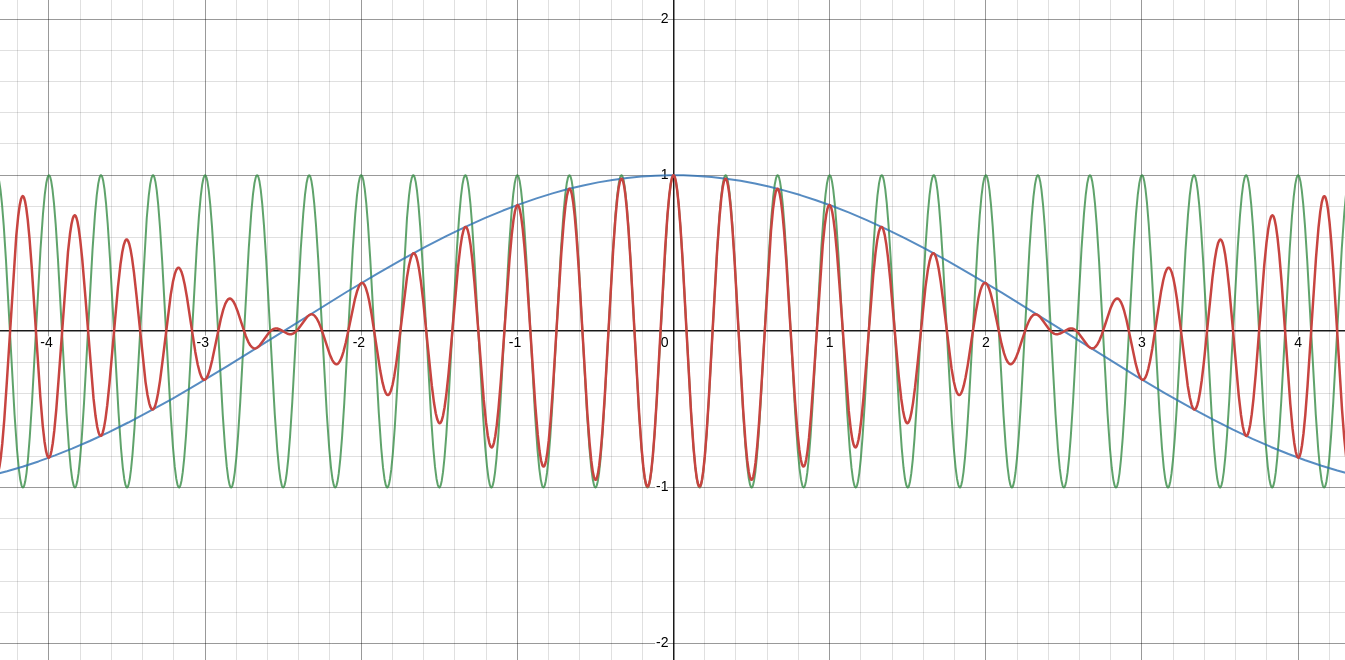
\includegraphics[width=0.48\textwidth]{fig/part-1/ex SA - 11.png}
	\hfill
	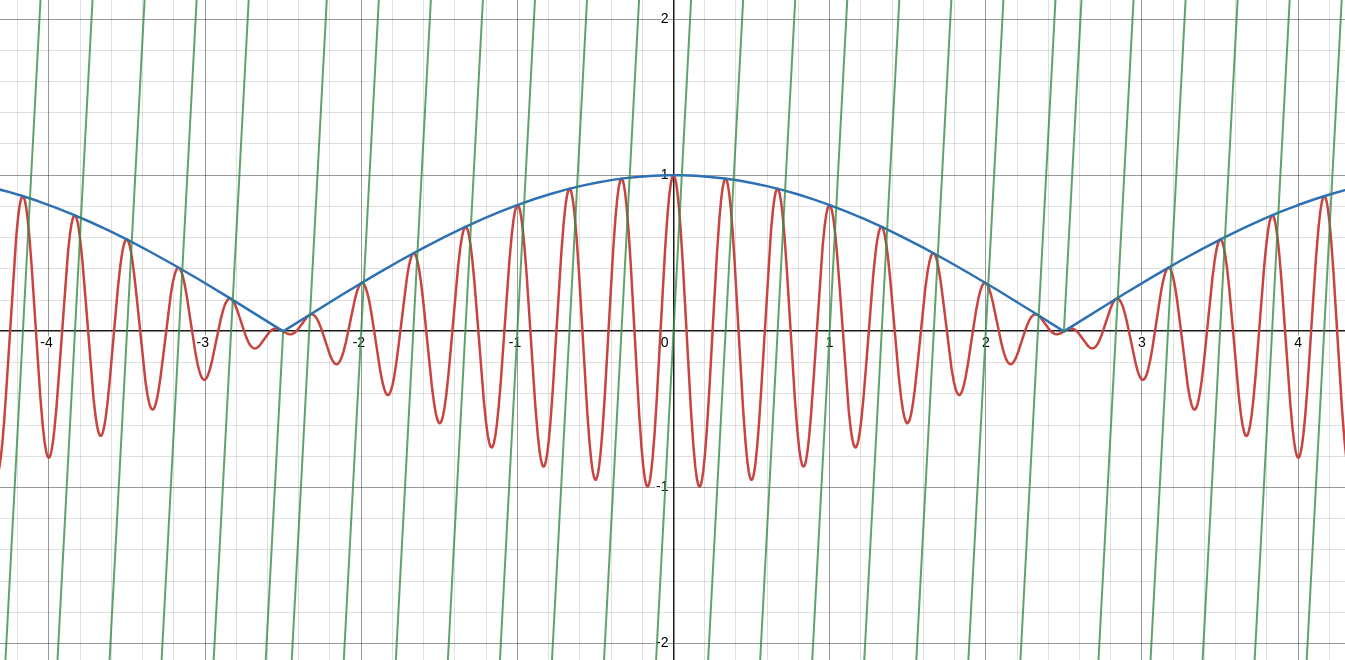
\includegraphics[width=0.48\textwidth]{fig/part-1/ex SA - 12.png}
	\caption{Représentation graphique du signal $x$ (rouge) avec $\nu_1=3$ et $\nu_2=0.1$. Sur l'image de gauche, avec signaux de fréquences pures (bleu et vert). Sur l'image de droite, avec son amplitude (bleu) et sa phase instantanée (vert). Les discontinuités de la phase sont dû à l'arrondi à $2\pi$  près de l'argument de $\SA{x_1}$ et à la façon dont il est calculé lorsque le signal s'annule (mise à 0). Voir \href{https://www.desmos.com/calculator/gcedcdfkhr}{ici} pour un graphique dynamique.}
	\label{fig:exemple_tSA_1/2}
\end{figure}

\noindent
On montre sans mal\footnote{\itshape
	$\fou{x}_1$ est donné par 4 Diracs, en ne gardant que ce non nul sur $\R^+$ on obtient le spectre de $\SA{x_1}$ et il reste plus qu'à inverser la transformée de Fourier.}
que si $\ \nu_1\geq\nu_2$, alors la transformée en SA de $x_1$ s'écrit :
\[\SA{x_1} = \cos \left(2\pi\nu_2 t\right) e^{2i \pi\nu_1 t}\]
\\
Le signal $\SA{x_1}$ n'est ici pas sous forme exponentielle à proprement parler puisque le cosinus peut être négatif (pour s'y ramener, il suffit de passer le cos en valeur absolue et d'ajouter $\pi$ à l'argument lorsque nécessaire) mais l’avantage de cette forme est qu'elle fait clairement apparaître les fréquences $\nu_{1,2}$. En particulier, la fréquence instantanée du signal est la plus grandes des deux fréquences $\nu_1$ et $\nu_2$. La plus petite, elle, se retrouve dans l'amplitude. 
\\
Ce résultat est rassurant en cela qu'il est plus naturel de voir le cosinus de basse fréquence comme modulant celui de haute fréquence que l'inverse comme on le voit sur la première image de la figure \ref{fig:exemple_tSA_1/2}. 
\\
Aussi, en mettant les hautes fréquences du signal dans la fréquence instantanée, on s'assure de limiter les variations de l'amplitude. Cela apporte bien plus de contrainte en terme de décomposition $(a_{x_1},\phi_{x_1})$, en cela qui si l'inverse étant vrai, alors toute les fréquences pourrait être envoyé dans l'amplitude, ce qui laisserait la phase invariante.
\\

Cela étant dit, lorsque l'on fait varier $\nu_1$ et $\nu_2$, le résultat n'est pas toujours si intuitif. C'est notamment le cas lorsque les deux deviennent de plus en plus proche :

\begin{figure}[h]\centering
	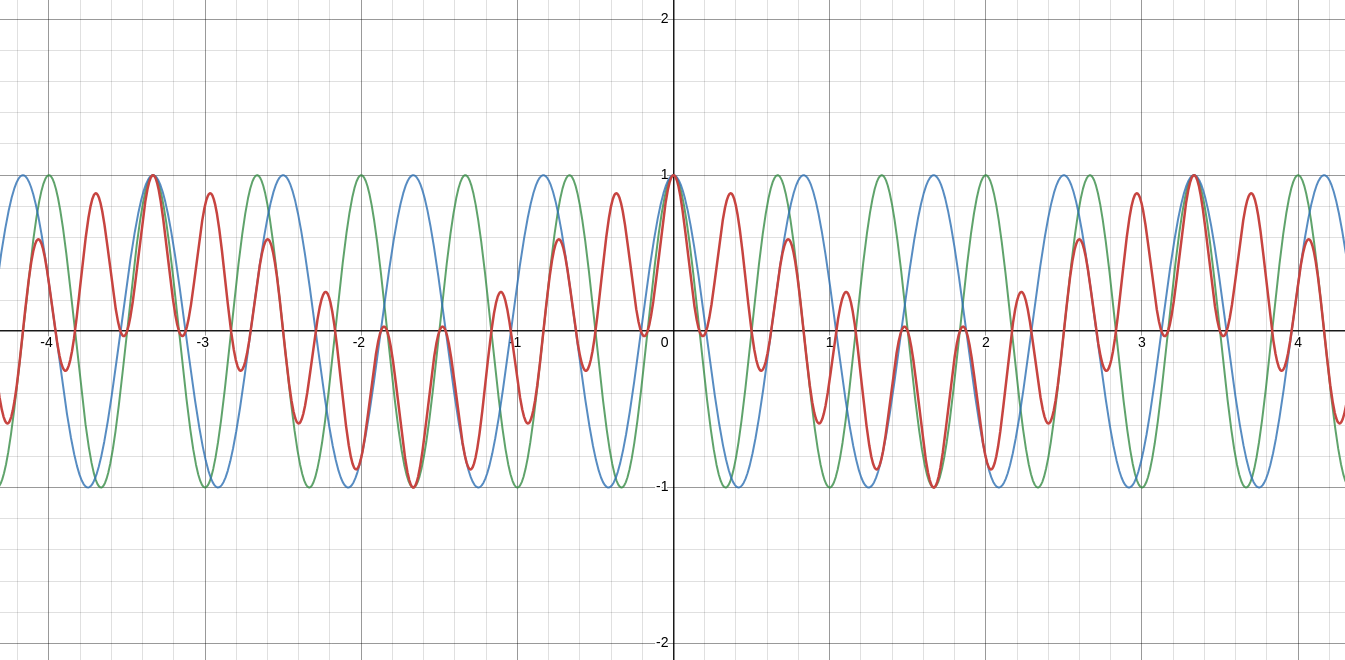
\includegraphics[width=0.48\textwidth]{fig/part-1/ex SA - 21.png}\hfill
	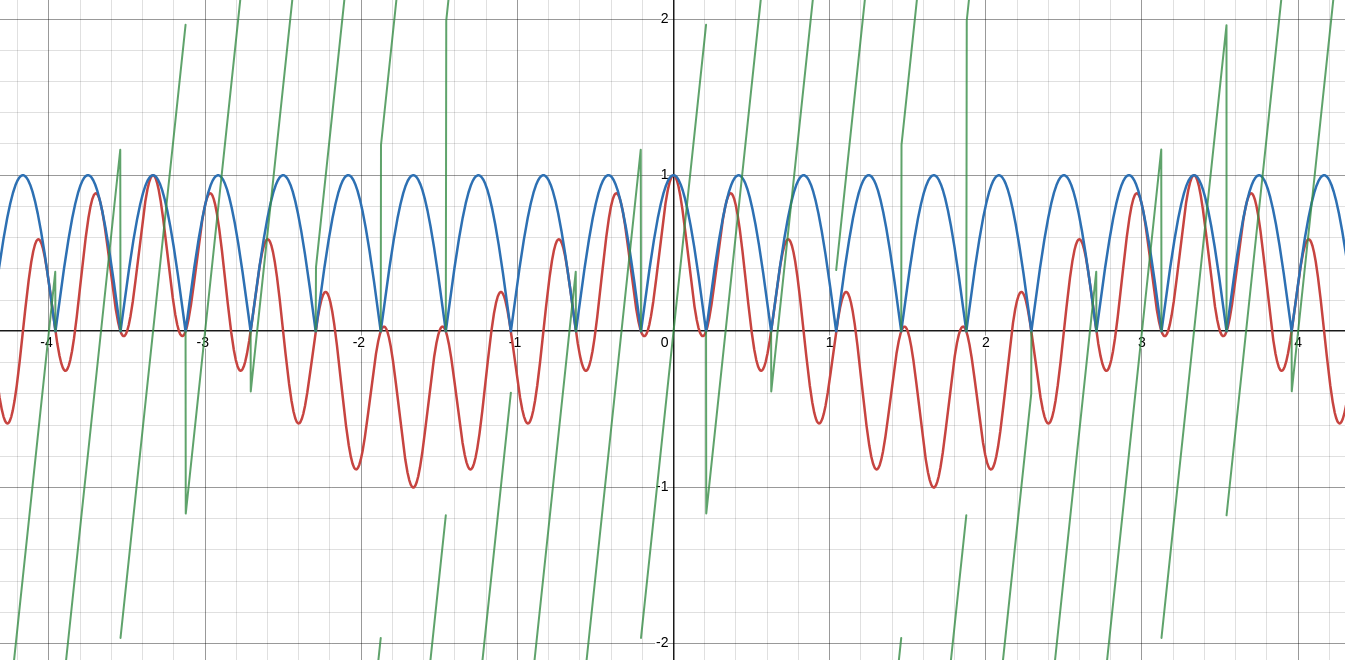
\includegraphics[width=0.48\textwidth]{fig/part-1/ex SA - 22.png}
	\caption{Idem que pour la figure \ref{fig:exemple_tSA_1/2} précédente, avec cette fois $\nu_1=1.5$ et $\nu_2=1.3$.}
	\label{fig:exemple_tSA_2/2}
\end{figure}

Pour comprendre pourquoi l'amplitude ne fait pas ce qu'on attendrait d'elle, est introduit le théorème de Bedrosian :

\begin{theoreme}[de Bedrosian]\label{theo:2Bedrosian}
	Dans sa formulation la plus générale, le théorème de Bedrosian énonce que si deux fonctions $f,g\in L^2(\R)$ sont telles l'une des trois assertions suivantes est vraie :
	\begin{itemize}%[label=\textit{\arabic*}. ]
		\item 
		\item $\exists \lambda\in\R^+\ |\ \supp \fou{f} \subset [-\lambda, +\infty[,\ \supp \fou{g} \subset [\lambda, +\infty[$\label{item:1condi_theo2Bedrosian}
		
		\item $\exists \lambda\in\R^+\ |\ \supp \fou{f} \subset ]-\infty, \lambda],\ \supp \fou{g} \subset ]-\infty,-\lambda]$ \label{item:2condi_theo2Bedrosian}
		
		\item $\exists (\lambda_1,\lambda_2)\in \R^+\times\R^+ \setminus\{(0,0)\}\ |\ \supp \fou{f} \subset [-\lambda_1, \lambda_2],\ \supp \fou{g} \subset \R\setminus[-\lambda_2,\lambda_1]$
		
	\end{itemize}
	alors la transformée de Hilbert de leur produit s'écrit (voir \cite{wang_simple_2009} pour une démonstration) :
	\begin{equation}\label{eq:2Bedrosian}
		\hilb{fg} = f\hilb{g}
	\end{equation}
\end{theoreme}

Dans le cas d'un signal réel, suivant la \cref{def:ampli-phase_instant} on peut écrire $\ x=a_x\cos \phi_x$.
Comme $a_x$ et $\cos \phi_x$ sont réelles, seule la troisième condition du théorème de Bedrosian peut être satisfaite pour peu que $\lambda_1=\lambda_2$. Ainsi :

\begin{corollaire}\label{coro:AM-FM}
	Toujours avec les même notations, si $a_x\in L^2(\R)$, $\cos\phi_x\in L^2(\R)$ et qu'il existe $\lambda\in\R^{+_*}$ tel que :
	\begin{equation}\label{eq:condiBedro_AM-FM}
		\supp \Fou{a_x} \subset [-\lambda, \lambda],\quad \supp \Fou{\cos\phi_x} \subset \R\setminus[-\lambda,\lambda]
	\end{equation}
	Alors on a :
	\begin{align}\label{eq:result_AM-FM}
		\hilb{x} &= a_x\hilb{\cos \phi_x}  &  \qquad\qquad&\text{et si }a_x(t)\neq 0,  &  \hilb{\cos \phi_x}(t) = \sin\phi_x(t)
	\end{align}
\end{corollaire}
\skipl

Pour interpréter ce \namecref{coro:AM-FM}, prenons un autre exemple : $\ x_2(t) = a(t)\cos(2\pi \nu_0 t)$. Sa transformé de Fourier est donnée par :
\begin{align*}
	\fou{x}_2(\nu) &= \fou{a}(\nu)*\frac{1}{2}\Big(\delta(\nu-\nu_0) + \delta(\nu+\nu_0)\Big) \\
	&= \frac{1}{2}\Big(\fou{a}(\nu+\nu_0) + \fou{a}(\nu-\nu_0)\Big)
\end{align*}
\\
Graphiquement, la transformé de Fourier de $x_2$ duplique le graphe de $\fou{a}$ en $\pm\nu_0$ et somme les deux. La condition \eqref{eq:condiBedro_AM-FM} du \cref{coro:AM-FM} demande alors que $\nu_0$ soit choisie de telle sorte que :
\[\supp \Fou{a}\subset[-\nu_0, \nu_0]\]
\\
C'est-à-dire qu'il n'y ait pas de chevauchement entre les deux courbes $\ \Gamma_\pm : \nu \longmapsto \fou{a}(\nu\mp\nu_0) $ (voir \cref{fig:alising-ish} ci-dessous). Moralement, cela assure qu'en ne prenant que la partie positive du spectre de $x_2$, l'on ne ramène pas avec une partie de $\fou{a}(\nu+\nu_0)$. Quant bien même cette explication est simpliste puisqu'ici $\phi$ est linaire, on peut voir que le phénomène est finalement très proche de celui d'aliasing.
\\

\begin{figure}[h]\centering
	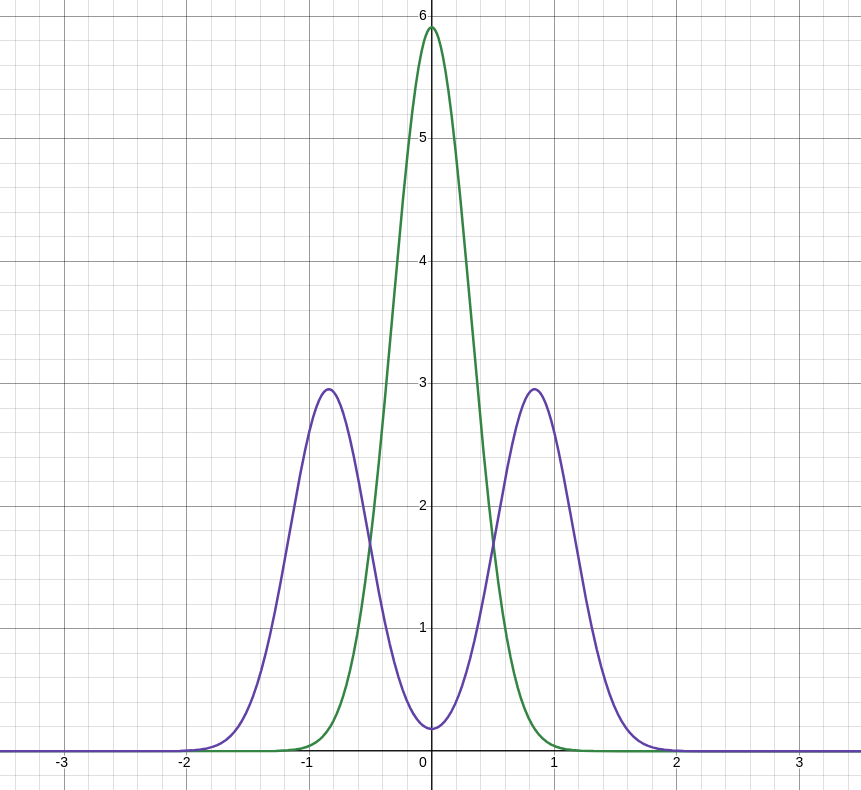
\includegraphics[width=0.45\textwidth]{fig/part-1/bedro condi 1.png} 
	\hfill
	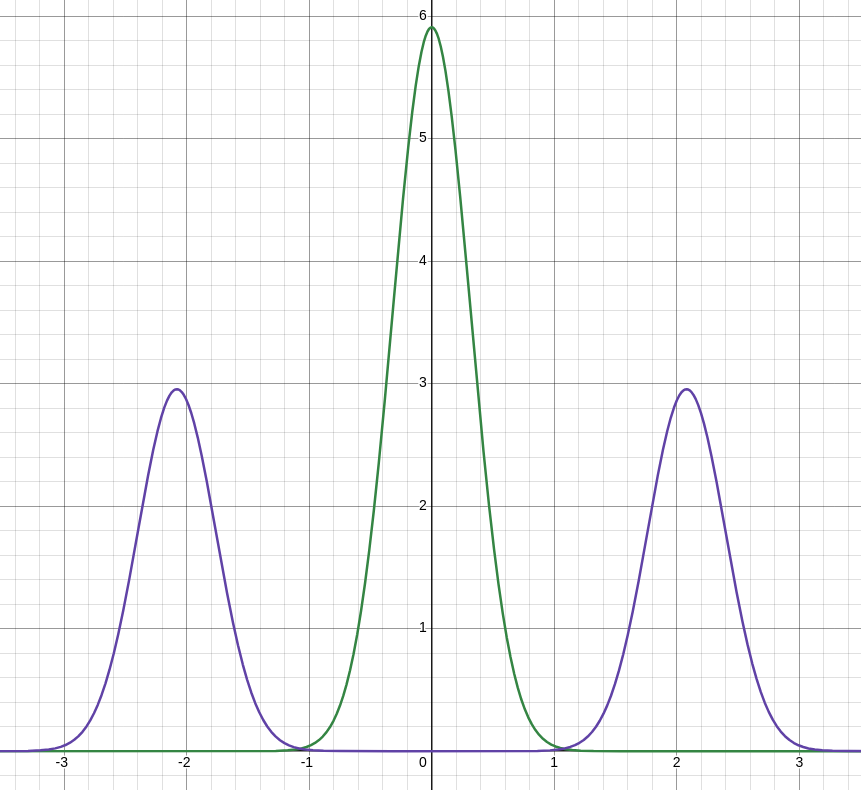
\includegraphics[width=0.45\textwidth]{fig/part-1/bedro condi 2.png} 
	\caption{Sur les deux graphiques sont représentés en vert $\fou{a}$ et en violet $\fou{x}_2$. Dans le premier cas l'hypothèse de Bedrosian et respectée mais pas dans le second.}
	\label{fig:alising-ish}
\end{figure}


Pour revenir sur l'exemple $x_1$ précédent, dans la seconde figure \ref{fig:exemple_tSA_2/2}, l'amplitude ne colle plus à l'interprétation que l'on voudrait justement parce que la condition de Bedrosian n'est plus respecter (à savoir $\nu_1\geq 2\nu_2$). 




\subsection{Calcul des phases}\label{ann:demo_phases_2var}

\begin{demo}[de la formule \eqref{eq:phaset_2var}, \cref{prop:phases_2var}]
	Pour la phase totale, on note cette fois $\mathcal{V} = \begin{pmatrix} \cos\chi \\ -i\sin\chi \end{pmatrix}$ et on a :
	\begin{align*}
		\big\langle \x(t), \x(t_0)\big\rangle &= \Big\langle a(t)e^{i\varphi(t)}R_{\theta(t)}\mathcal{V}(t), a(t_0)e^{i\varphi(t_0)}R_{\theta(t_0)}\mathcal{V}(t_0) \Big\rangle \\
		&= a(t)e^{i\varphi(t)} a(t_0)e^{-i\varphi(t_0)} \Big\langle R_{\theta(t)}\mathcal{V}(t), R_{\theta(t_0)}\mathcal{V}(t_0) \Big\rangle \\
		%&= a(t_0)a(t)e^{i(\varphi(t_0)-\varphi(t))}\Big\langle \mathcal{V}(t_0), R_{\theta(t_0)}^{-1}R_{\theta(t)}\mathcal{V}(t) \Big\rangle \\
		&= a(t_0)a(t)e^{i(\varphi(t)-\varphi(t_0))}\Big\langle R_{\theta(t)- \theta(t_0)}\mathcal{V}(t), \mathcal{V}(t_0) \Big\rangle
	\end{align*}
	Pour alléger les notations, on note $\ \Delta y =y(t)-y(t_0)$, $\ y_1=y(t_0)\ $ et $\ y_2=(t)\ $ pour $\ y=\varphi,\theta,\chi$. Le produit hermitien à droite s'écrit alors :
	\begin{align*}
		\Big\langle R_{\Delta\theta}\mathcal{V}(t), \mathcal{V}(t_0) \Big\rangle &=   \Big(\cos\Delta\theta \cos\chi_2 + i\sin\Delta\theta \sin\chi_2 \qquad \sin\Delta\theta \cos\chi_2 - i\cos\Delta\theta \sin\chi_2\Big) \begin{pmatrix} \cos\chi_1 \\ i\sin\chi_1 \end{pmatrix} \\
		&= \cos\chi_1\Big(\cos\Delta\theta \cos\chi_2 + i\sin\Delta\theta \sin\chi_2\Big) + i\sin\chi_1\Big(\sin\Delta\theta \cos\chi_2 - i\cos\Delta\theta \sin\chi_2\Big) \\
		&= \cos\Delta\theta \Big(\cos\chi_1 \cos\chi_2 + \sin\chi_1 \sin\chi_2\Big) + i\sin\Delta\theta \Big( \cos\chi_1 \sin\chi_2 + \sin\chi_1\cos\chi_2\Big) \\
		&= \cos\Delta\theta \cos\Delta\chi + i\sin\Delta\theta \sin(\chi_1+\chi_2)
	\end{align*}
	\\
	D'où la phase totale :
	\begin{align*}
		\phaset(\x) = \arg\big\langle \x(t), \x(t_0)\big\rangle &= \arg\left( a(t_0)a(t)e^{i(\varphi(t) - \varphi(t_0))}\Big( \cos\Delta\theta \cos\Delta\chi + i\sin\Delta\theta \sin(\chi_1+\chi_2) \Big) \right) \\
		&= \varphi(t) - \varphi(t_0) + \arg\Big( \cos\Delta\theta \cos\Delta\chi + i\sin\Delta\theta \sin(\chi_1+\chi_2) \Big)
	\end{align*}
	et l'argument restant s'écrit comme une arctangente, donnant :
	\begin{align*}
		\phaset(\x) &= \varphi(t)-\varphi(t_0) + \arctan\frac{\sin\Delta\theta \sin(\chi_1+\chi_2)}{\cos\Delta\theta \cos\Delta\chi} \\
		&= \varphi(t)-\varphi(t_0) + \arctan \left( \tan\Delta\theta\frac{\sin(\chi_1+\chi_2)}{\cos\Delta\chi} \right) \\
		&= \cdots
	\end{align*}
\end{demo}

\begin{demo}[de la formule \eqref{eq:phased_2var}, \cref{prop:phases_2var}]
	Par souci de lisibilité, on note $\ \mathcal{U} = R_{\theta} \begin{pmatrix} \cos\chi \\ -i\sin\chi \end{pmatrix} = \begin{pmatrix} \cos\theta(t) \cos\chi(t) + i\sin\theta(t) \sin\chi(t) \\ \sin\theta(t) \cos\chi(t) - i\cos\theta(t) \sin\chi(t) \end{pmatrix}$, de sorte que la dérivée de $\ \x=ae^{i\varphi}\mathcal{U}\ $ s'écrive :
	\[\dot{\x} = a'e^{i\varphi}\mathcal{U} + ia\varphi'e^{i\varphi} \mathcal{U} + ae^{i\varphi}\theta'\begin{pmatrix} -\sin\theta \cos\chi + i\cos\theta \sin\chi \\ \cos\theta \cos\chi + i\sin\theta \sin\chi \end{pmatrix} + ae^{i\varphi}\chi'\begin{pmatrix} -\cos\theta \sin\chi + i\sin\theta \cos\chi \\ -\sin\theta \sin\chi - i\cos\theta \cos\chi \end{pmatrix}\]
	\\
	Les vecteurs des deux derniers membres s'expriment en fonction des composantes $\ \mathcal{U}_{1,2}\ $ de $\ \mathcal{U}$ :
	\begin{align*}
		\begin{pmatrix} -\sin\theta \cos\chi + i\cos\theta \sin\chi \\ \cos\theta \cos\chi + i\sin\theta \sin\chi \end{pmatrix} &= \begin{pmatrix} -\mathcal{U}_2 \\ \mathcal{U}_1 \end{pmatrix}  &
		\begin{pmatrix} -\cos\theta \sin\chi + i\sin\theta \cos\chi \\ -\sin\theta \sin\chi - i\cos\theta \cos\chi \end{pmatrix} &= i\begin{pmatrix} \congu{\mathcal{U}}_2 \\ -\congu{\mathcal{U}}_1 \end{pmatrix}
	\end{align*}
	\\
	Le produit hermitien $\langle \dot{\x}, \x \rangle$ s'écrit alors :
	\begin{align*}
		\langle \dot{\x}, \x \rangle 
		&= \left\langle a'e^{i\varphi}\mathcal{U} + ia\varphi'e^{i\varphi} \mathcal{U} + ae^{i\varphi}\theta'\begin{pmatrix} -\mathcal{U}_2 \\ \mathcal{U}_1 \end{pmatrix} + iae^{i\varphi}\chi'\begin{pmatrix} \congu{\mathcal{U}}_2 \\ -\congu{\mathcal{U}}_1 \end{pmatrix}, ae^{i\varphi}\mathcal{U} \right\rangle \\
		&= \left\langle a'\mathcal{U} + ia\varphi' \mathcal{U} + a\theta'\begin{pmatrix} -\mathcal{U}_2 \\ \mathcal{U}_1 \end{pmatrix} + ia\chi'\begin{pmatrix} \congu{\mathcal{U}}_2 \\ -\congu{\mathcal{U}}_1 \end{pmatrix}, a\mathcal{U} \right\rangle \\
		&= aa' \big\langle \mathcal{U}, \mathcal{U}\big\rangle  + ia^2\varphi' \big\langle \mathcal{U}, \mathcal{U}\big\rangle  + a^2\theta'\left\langle \begin{pmatrix} -\mathcal{U}_2 \\ \mathcal{U}_1 \end{pmatrix}, \mathcal{U} \right\rangle + ia^2\chi'\left\langle \begin{pmatrix} \congu{\mathcal{U}}_2 \\ -\congu{\mathcal{U}}_1 \end{pmatrix}, \mathcal{U} \right\rangle
	\end{align*}
	où les deux derniers produits hermitiens donnent :
	\begin{align*}
		\left\langle \begin{pmatrix} -\mathcal{U}_2 \\ \mathcal{U}_1 \end{pmatrix}, \mathcal{U} \right\rangle &= -\mathcal{U}_2\congu{\mathcal{U}}_1 + \mathcal{U}_1\congu{\mathcal{U}}_2 \\
		&= 2i\Im m\big(\mathcal{U}_1 \congu{\mathcal{U}}_2\big) \\
		&= 2i\Im m\Big(\big( \cos\theta \cos\chi + i \sin\theta \sin\chi \big) \big( \sin\theta \cos\chi + i \cos\theta \sin\chi \big)\Big) \\
		&= 2i\big(\cos^2\theta \cos\chi \sin\chi + \sin^2\theta \sin\chi \cos\chi \big) \\
		&= 2i \cos\chi \sin\chi \\
		&= i\sin2\chi 
		\\ \\
		\left\langle \begin{pmatrix} \congu{\mathcal{U}}_2 \\ -\congu{\mathcal{U}}_1 \end{pmatrix}, \mathcal{U} \right\rangle &= \congu{\mathcal{U}_2\mathcal{U}_1} - \congu{\mathcal{U}_1\mathcal{U}_2} = 0
	\end{align*}
	\\
	D'où, sachant que $\ \|\x\|^2=a^2\ $ et $\ \|\mathcal{U}\|=1$, la formule :
	\begin{align*}
		\frac{\Im m\big\langle \dot{\x}, \x\big\rangle}{\|\x\|^2} &= \frac{1}{a^2}\Im m\Big(aa' \big\langle \mathcal{U}, \mathcal{U}\big\rangle  + ia^2\varphi' \big\langle \mathcal{U}, \mathcal{U}\big\rangle + ia^2\theta' \sin2\chi \Big) \\
		&= \frac{1}{a^2} \Big( a^2\varphi' \|\mathcal{U}\|^2 + a^2\theta' \sin2\chi \Big) \\
		&= \varphi' + \theta' \sin2\chi
	\end{align*}
\end{demo}
\skipl


\subsection{\todo Lien entre Poincaré et Bloch (EN VRAC)}

\thoughts{Un paquet de calculs, comme pour l'annexe A, il faudra que je le remette en forme , remette du contexte et que j'enlève des choses.}



\subsubsection{\todo Lien entre les deux types de signaux}

Soit le signal :
\[\x_B(\varphi, \theta, \chi) = e^{i\varphi} \begin{pmatrix}
	\cos \chi/2 \\ e^{i\theta}\sin\chi/2\end{pmatrix}\]
Pour le réécrire en terme de vecteur AM-FM-PM, il faut faire apparaître une matrice de rotation, matrice qui est diagonalisable dans $\C^{n\times n}$ via la relation :
\begin{align*}
	&\begin{pmatrix} 
		\cos \alpha & -\sin \alpha \\ 
		\sin\alpha & \cos\alpha 
	\end{pmatrix} = \frac{1}{2} \begin{pmatrix} 
		1 & -1 \\ i & i
	\end{pmatrix}\begin{pmatrix} 
		e^{-i\alpha} & 0 \\ 
		0 & e^{i\alpha} 
	\end{pmatrix}\begin{pmatrix} 
		1 & -i \\ -1 & -i
	\end{pmatrix}\\
	&\Llr\quad \begin{pmatrix} 
		1 & -i \\ -1 & -i
	\end{pmatrix}\begin{pmatrix} 
		\cos \alpha & -\sin \alpha \\ 
		\sin\alpha & \cos\alpha 
	\end{pmatrix} \begin{pmatrix} 
		1 & -1 \\ i & i
	\end{pmatrix} = 2 \begin{pmatrix} 
		e^{-i\alpha} & 0 \\ 
		0 & e^{i\alpha} 
	\end{pmatrix}
\end{align*}
\\
Cela permet d'écrire :
\begin{align*}
	\x_B(\varphi, \theta, \chi) &= e^{i\varphi} e^{i\theta/2}\begin{pmatrix}
		e^{-i\theta/2} & 0 \\
		0 & e^{i\theta/2}
	\end{pmatrix}\begin{pmatrix} 
		\cos \chi/2 \\ 
		\sin \chi/2 
	\end{pmatrix} \\
	&= \frac{1}{2}e^{i\varphi} e^{i\theta/2}\begin{pmatrix} 
		1 & -i \\
		-1 & -i
	\end{pmatrix}\begin{pmatrix} 
		\cos \theta/2 & -\sin \theta/2 \\ 
		\sin \theta/2 & \cos \theta/2 
	\end{pmatrix} \begin{pmatrix} 
		1 & -1 \\ i & i
	\end{pmatrix}\begin{pmatrix} 
		\cos \chi/2 \\ 
		\sin\chi/2
	\end{pmatrix} \\
	&= \frac{\sqrt{2}}{2}e^{i(\varphi + \theta/2)}U R_{\theta/2} \begin{pmatrix} 
		\cos \chi/2 - \sin\chi/2 \\ 
		i\big(\cos\chi/2 + \sin\chi/2\big)
	\end{pmatrix}   & &\text{où }\quad U = \frac{\sqrt{2}}{2}\begin{pmatrix} 
		1 & -i \\ -1 & -i
	\end{pmatrix}\in \U{2} \\
\end{align*}
\\
Ensuite, pour réduire les sommes dans le vecteur de droite, on a rappel les formules :
\begin{align*}
	\cos\left( \frac{\pi}{2} \pm \alpha\right) &= \frac{\sqrt{2}}{2}\big( \cos\alpha \mp \sin \alpha \big) & \sin\left( \frac{\pi}{2} \pm \alpha\right) &= \frac{\sqrt{2}}{2}\big( \cos\alpha \pm \sin \alpha \big)
\end{align*}
\\ 
On a donc deux choix pour chaque composante du vecteur mais celle avec un signe moins son préférable sachant que : 
\begin{align*}
	\cos\left( \frac{\pi}{2} - \alpha\right) &= \sin(\alpha) &  \sin\left( \frac{\pi}{2} - \alpha\right) &= \cos(\alpha)
\end{align*}
\\
On choisi donc la seconde formule pour la première composante et la premier pour la seconde composante, donnant :
\begin{align*}
	\x_B(\varphi, \theta, \chi) &= \frac{\sqrt{2}}{2}e^{i(\varphi + \theta/2)}U R_{\theta/2} \begin{pmatrix} 
		\cos \chi/2 - \sin\chi/2 \\ 
		i\big(\cos\chi/2 + \sin\chi/2\big)
	\end{pmatrix} \\
	&= e^{i(\varphi + \theta/2)}U R_{\theta/2} \begin{pmatrix} 
		\sin\left( \frac{\pi}{2} - \chi/2\right) \\ 
		i\cos\left( \frac{\pi}{2} - \chi/2\right)
	\end{pmatrix} \\
	&= e^{i(\varphi + \theta/2)}U R_{\theta/2} \begin{pmatrix} 
		\cos \chi/2 \\ 
		i\sin \chi/2
	\end{pmatrix}
\end{align*}
\\
Ne reste alors plus qu'à ajuster les signes pour obtenir une écriture de signal $\x_P$ AM-FM-PM :
\begin{align*}
	\x_B(\varphi, \theta, \chi) &= e^{i(\varphi + \theta/2)}U R_{\theta/2} \begin{pmatrix} 
		\cos \chi/2 \\ 
		i\sin \chi/2
	\end{pmatrix} \\
	&= U e^{i(\varphi + \theta/2)} R_{\theta/2} \begin{pmatrix} 
		\cos (-\chi/2) \\ 
		-i\sin (-\chi/2)
	\end{pmatrix}
\end{align*}
En somme :
\begin{align} \label{eq:bloch2poinca}
	\x_B(\psi, \alpha, \beta) &= U \x_P(\psi + \alpha/2, \alpha/2, -\beta/2)  & 
	\x_P(\varphi, \theta, \chi) = U^\dagger 	\x_B(\varphi-\theta, 2\theta, -2\chi)	
\end{align}
\skipl 



\subsubsection{\todo Lien entre les projections}

Avec la formule \eqref{eq:bloch2poinca} ci-dessus, on a :

\begin{align}
	\rho_B(\alpha, \beta) &= U \rho_P(\alpha/2, -\beta/2)U^\dagger  & 
	\rho_P(\theta, \chi) &= U^\dagger \rho_B(2\theta, -2\chi) U
	%\\ \Llr\ \rho_B(\alpha, \beta) U &= U \rho_P(\alpha/2, -\beta/2) & \Llr\ \rho_P(\theta, \chi) U^\dagger &= U^\dagger \rho_B(2\theta, -2\chi) 
\end{align}
\\
Mais on a aussi, dans la base Pauli :
\begin{align*}
	\sigma_1 &= \begin{pmatrix} 0 & 1 \\ 1 &  0 \end{pmatrix}  &
	\sigma_2 &= \begin{pmatrix} 0 & -i \\  i &  0 \end{pmatrix}  &
	\sigma_3 &= \begin{pmatrix} 1 & 0 \\ 0 & -1 \end{pmatrix}
\end{align*}
les expressions :
\begin{align*}
	\rho_{P}(\theta, \chi) &= \frac{1}{2} \Big( id + \sin(2\theta) \cos(2\chi) \sigma_1 - \sin (2\chi) \sigma_2 + \cos(2\theta) \cos(2\chi) \sigma_3 \Big) \\ 
	\rho_{B}(\alpha, \beta) &= \frac{1}{2} \Big( id + \cos(\alpha) \sin(\beta) \sigma_1 + \sin(\alpha) \sin(\beta) \sigma_2 + \cos (\beta) \sigma_3 \Big)
\end{align*}
\skipl

Pour les lier, on pose $\ 2\theta = \nicefrac{\pi}{2} - \alpha\ $ et $\ 2\chi = \nicefrac{\pi}{2} - \beta$, donnant :
\begin{align*}
	\rho_P(\theta, \chi) - id 
	&= \sin(\nicefrac{\pi}{2} - \alpha) \cos(\nicefrac{\pi}{2} - \beta) \sigma_1 - \sin (\nicefrac{\pi}{2} - \beta) \sigma_2 + \cos(\nicefrac{\pi}{2} - \alpha) \cos(\nicefrac{\pi}{2} - \beta) \sigma_3 \\
	&= \cos(\alpha) \sin(\beta) \sigma_1 - \cos (\beta) \sigma_2 + \sin(\alpha) \sin(\beta) \sigma_3
\end{align*}
\\
Ce qui sous forme matricielle se réécrit :
\[\begin{pmatrix}
	\sin(2\theta) \cos(2\chi) \\ -\sin (2\chi) \\ \cos(2\theta) \cos(2\chi)
\end{pmatrix} = \begin{pmatrix}
	\cos(\alpha) \sin(\beta) \\ -\cos (\beta) \\ \sin(\alpha) \sin(\beta)
\end{pmatrix} = \begin{pmatrix}
	1 & 0 & 0 \\ 0 & 0 & -1 \\ 0 & 1 & 0
\end{pmatrix}\begin{pmatrix}
	\cos(\alpha) \sin(\beta) \\ \sin(\alpha) \sin(\beta) \\ \cos (\beta)
\end{pmatrix}\]
\\
Donc la passage de $\rho_B$ à $\rho_S$ se fait via un changement et d'angle et une rotation de $\nicefrac{\pi}{2}$ autour de $\sigma_1$.
\\

Même calcul, cette fois, en partant de \eqref{eq:bloch2poinca} :
\begin{align*}
	2\rho_P(\theta, \chi) &= 2U^\dagger \rho_B(2\theta, -2\chi) U \\
	&= U^\dagger \Big( id + \cos(2\theta) \sin(-2\chi) \sigma_1 + \sin(2\theta) \sin(-2\chi) \sigma_2 + \cos (-2\chi) \sigma_3 \Big) U \\
	&= id - \cos(2\theta) \sin(2\chi) U^\dagger \sigma_1 U - \sin(2\theta) \sin(2\chi) U^\dagger \sigma_2 U + \cos (2\chi) U^\dagger \sigma_3 U
\end{align*}
avec :
\begin{align*}
	U^\dagger \sigma_1 U &= \frac{1}{2} \begin{pmatrix} 
		1 & -1 \\ i & i
	\end{pmatrix} \begin{pmatrix} 
		0 & 1 \\ 1 &  0 
	\end{pmatrix} \begin{pmatrix} 
		1 & -i \\ -1 & -i
	\end{pmatrix} = \frac{1}{2} \begin{pmatrix} 
		-2 & 0 \\ 0 & 2
	\end{pmatrix} = -\sigma_3 \\
	U^\dagger \sigma_2 U &= \frac{1}{2} \begin{pmatrix} 
		1 & -1 \\ i & i
	\end{pmatrix} \begin{pmatrix} 
		0 & -i \\  i &  0 
	\end{pmatrix} \begin{pmatrix} 
		1 & -i \\ -1 & -i
	\end{pmatrix} = \frac{1}{2} \begin{pmatrix} 
		0 & -2 \\ -2 & 0
	\end{pmatrix} = -\sigma_1 \\
	U^\dagger \sigma_3 U &= \frac{1}{2} \begin{pmatrix} 
		1 & -1 \\ i & i
	\end{pmatrix}  \begin{pmatrix} 
		1 & 0 \\ 0 & -1 
	\end{pmatrix} \begin{pmatrix} 
		1 & -i \\ -1 & -i
	\end{pmatrix} = \frac{1}{2} \begin{pmatrix} 
		0 & -2i \\ 2i & 0
	\end{pmatrix} = \sigma_2
\end{align*}
\\
Qui donne :
\begin{align*}
	2\rho_P(\theta, \chi) &= id - \cos(2\theta) \sin(2\chi) U^\dagger \sigma_1 U - \sin(2\theta) \sin(2\chi) U^\dagger \sigma_2 U + \cos (2\chi) U^\dagger \sigma_3 U \\
	&= id + \cos(2\theta) \sin(-2\chi) \sigma_3 + \sin(2\theta) \sin(-2\chi)  \sigma_1 + \cos (-2\chi) \sigma_2 \\
	&= id + \sin(2\theta) \sin(2\chi)  \sigma_1 + \cos (2\chi) \sigma_2 + \cos(2\theta) \sin(2\chi) \sigma_3
\end{align*}
\\ 
Le tout reste cohérent et avec les notations :
\begin{align*}
	w_P(\theta, \chi) &= \begin{pmatrix}
		\sin(\theta) \cos(\chi) \\ -\sin (\chi) \\ \cos(\theta) \cos(\chi)
	\end{pmatrix}  &   w_B\big( \alpha, \beta \big) = \begin{pmatrix}
		\cos(\alpha) \sin(\beta) \\ \sin(\alpha) \sin(\beta) \\ \cos (\beta)
	\end{pmatrix}
\end{align*}
Cela devient :
\[w_P(2\theta, 2\chi) = \begin{pmatrix}
	1 & 0 & 0 \\ 0 & 0 & -1 \\ 0 & 1 & 0
\end{pmatrix} w_B\big( (\nicefrac{\pi}{2}-\theta ), \big(\nicefrac{\pi}{2}-\chi) \big)\]
\skipl 



\subsubsection{\todo Transformation de phases}

Première chose, le produit hermitien est invariant par $U\in\U{2}$ (si si). Ainsi :
\[\big\langle U\x(t_0), U\x(t) \big\rangle = \big\langle \x(t_0), \x(t) \big\rangle\]
\[\big\langle (U\x)', U\x \big\rangle = \big\langle U\x', U\x \big\rangle = \big\langle \x', \x \big\rangle\]
\\
Ainsi, en utilisant les formules \eqref{eq:phaset_2var} et \eqref{eq:bloch2poinca}, on a :
\begin{align*}\phaset \big(\x_B(\psi, \alpha, \beta) \big) &= \phaset \big(\x_P(\psi + \alpha/2, \alpha/2, -\beta/2) \big) \\
	&= \big( \psi + \alpha/2 \big)(t) - \big( \psi + \alpha/2 \big)(t_0) - \arctan\left( \tan \frac{\Delta\theta}{2} \frac{ \tan 2\beta(t_0)+\tan 2\chi(t)}{1 + \tan 2\beta(t_0)\tan 2\beta(t)}\right)
\end{align*}
Mais avec un calcul immédiat, on a aussi :
\[aoerinagrqobne\]
\\
Avec la formule de la phase dynamique dans Poincaré \eqref{eq:phased_2var}, on a :
\begin{align*}
	%\phaset \big(\x_B(\psi, \alpha, \beta) \big) &= \phaset \big(\x_P(\psi + \alpha/2, \alpha/2, -\beta/2) \big) 
	%\\ \\
	\phased \big(\x_B(\psi, \alpha, \beta) \big) &= \Im m \int_{t_0}^t \left\langle \frac{d}{ds}\x_B(\psi, \alpha, \beta), \x_B(\psi, \alpha, \beta) \right\rangle ds \\
	&= \Im m \int_{t_0}^t \left\langle \frac{d}{ds}\x_P(\psi + \alpha/2, \alpha/2, -\beta/2), \x_P(\psi + \alpha/2, \alpha/2, -\beta/2) \right\rangle ds \\
	&= \phased \big( \x_P(\psi + \alpha/2, \alpha/2, -\beta/2) \big) \\
	&= \psi(t) + \alpha(t)/2 - \big( \psi(t_0) + \alpha(t_0)/2 \big) - \int_{t_0}^t \frac{\alpha'(s)}{2} \sin \big( -2\beta(s)/2 \big) ds \\
	&= \psi(t) - \psi(t_0) + \frac{\alpha(t) - \alpha(t_0)}{2} + \frac{1}{2} \int_{t_0}^t \alpha'(s)\sin \beta(s) ds
\end{align*}
\\
Mais dans le même temps, si on calcul la phase dynamique de $\x_B$, on tombe cette fois sur :
\begin{align*}
	\phased\big(\x_B(\psi, \alpha, \beta) \big) &= \psi(t) - \psi(t_0) +  \int_{t_0}^t \alpha'(s) \frac{1 - \cos\beta(s)}{2}ds \\
	&= \psi(t) - \psi(t_0) + \frac{\alpha(t) - \alpha(t_0)}{2}- \frac{1}{2} \int_{t_0}^t \alpha'(s) \cos\beta(s) ds 
\end{align*}
Auquel cas :
\begin{align*}
	\phased\big(\x_S(\varphi, \theta, \chi) \big) &= \phased\big(\x_B(\varphi-\theta, 2\theta, -2\chi) \big) \\
	&= \varphi(t) - \theta(t) - \big( \varphi(t_0) - \theta(t_0) \big) + \frac{1}{2} \int_{t_0}^t 2\theta' (1 - \cos2\chi)ds \\
	&= \varphi(t) - \varphi(t_0) - \big( \theta(t) - \theta(t_0) \big) + \int_{t_0}^t \theta' (1 - \cos2\chi)ds \\
	&= \varphi(t) - \varphi(t_0) - \big( \theta(t) - \theta(t_0) \big) + \big( \theta(t) - \theta(t_0) \big) - \int_{t_0}^t \theta' \cos2\chi ds \\
	&= \varphi(t) - \varphi(t_0) - \int_{t_0}^t \theta' \cos2\chi ds
\end{align*}
Ce qui voudrait dire que :
\[\phased\big(\x_S(\varphi, \theta, \chi) \big) = \varphi(t) - \varphi(t_0) + \int_{t_0}^t \theta' \sin2\chi ds = \varphi(t) - \varphi(t_0) - \int_{t_0}^t \theta' \cos2\chi ds\]
... bizarre